\documentclass{llncs}

\usepackage[utf8x]{inputenc}
\usepackage[english,russian]{babel}
\usepackage{cmap}
\usepackage{dsfont}
\usepackage{amsmath}
\usepackage{comment}
\usepackage{graphicx}
\usepackage{caption}

\pagestyle{plain}

\title{Гауссовские процессы для активного \\ обучения в задаче классификации}
\author{Дарья Котова\inst{1}, Максим Панов\inst{2}}
\institute{1: Московский физико-технический институт (ГУ) \\ \email{kotova.ds@phystech.edu} \\
2: Сколковский институт науки и технологий \\ \email{m.panov@skoltech.ru}}
%\email {kotova.ds@phystech.edu}, 
%\inst{2} Сколковский институт науки и технологий
%\email {m.panov@skoltech.ru}}

\begin{document}

\maketitle
%контакты Панова, объем текста, вставить картинки, score

\begin{abstract}

Активное обучение -- новый подход к обучению моделей, который основывается на адаптивном увеличении обучающей выборки ранее неразмеченными точками. Как правило выбор точек основан на оценке неопределенности предсказания модели в точки. Гауссовский процесс -- стохастический процесс, такой что любой конечный набор этих случайных величин имеет многомерное нормальное распределение. \\
Недавно был предложен новый критерий для алгоритма активного обучения \cite{av}, с приложением так же и для гауссовских процессов. Критерий оценивает норму функции, которая описывает тренировочное множество в совокупности с еще одной неотмеченной точкой. Предполагается, что неотмеченная точка, дающая максимальную норму, несет больше информации о данных в целом. В этой работе исследуются различные варианты этого критерия. 

\end{abstract}

\begin{center}
{\bfseries Ключевые слова: } активное обучение, гауссовские процессы
\end{center}
%Нейронные сети с большим количеством параметров обладают хорошим обобщающим свойством и до %сих пор непонятно, почему \cite{overparam}. Пониманию этого вопроса, возможно, %поспособствует изучение другого класса моделей -- гауссовских процессов. \\
\section{Введение}
В последнее время, возрастает интерес к активному обучению \cite{generalav} -- новому подходу к обучению, который позволит сократить размеры обучающей выборки. Недавно был предложен новый критерий для алгоритма активного обучения \cite{av}, разработанный в рассмотрении нейронных сетей с большим количеством параметров. Под последними имеются в виду такие модели, что отношения числа параметров $p$ к размеру обучащей выборки $n$ стремится к константе, большей единицы, при стремлении $p$ и $n$ к бесконечности. В этой работе исследуются различные варианты этого алгоритма, с той разницей, что вместо нейронных сетей ипользуются гауссовские процессы. Интуитивно, их связь можно объяснить следующим образом: выход слоя нейронной сети -- есть линейная комбинация входов. Если считать признаки независимыми, а количество нейронов в слое достаточно большим, то имеет место центральная предельная теорема \cite{teorver}, которая утверждает, что сумма достаточно большого количества слабо зависимых случайных величин, имеет распределение, близкое к нормальному. Гауссовский процесс же -- бесконечно число случайных величин, любая конечная комбинация которых имеет нормальное распределение. Таким образом, есть связь между гауссовскими процессами и нейронными сетями с большим количеством параметров. В этой работе мы сосредоточимся на гауссовских процессах, а в будущем планируем заняться нейронными сетями.
\section{Гауссовские процессы и их применение к задаче классификации}
Здесь мы кратко введем некоторые необходимые для работы с ними определения. Полный обзор гауссовских процессов и их свойств представлен в \cite{gp}.
\spnewtheorem{defi}{Определение}{\bfseries}{\em}
\begin{defi}
Гауссовский процесс $f\left(x\right)$ -- стохастический процесс (совокупность случайных величин, индексированных некоторым параметром, чаще всего временем или координатами), такой что любой конечный набор этих случайных величин имеет многомерное нормальное распределение.
\end{defi}
Здесь в нашем случае $x \in \bbbr^D$, где $D$ - произвольное натуральное число.
Гауссовский процесс полностью определяется функцией среднего и ковариационной функцией. Часто для упрощения записи функция среднего выбирается константой, равной 0. Введем обозначения:
\begin{equation}
m\left(x\right) = \mathds{E}\left[ f\left(x\right) \right] = 0,
\end{equation}
\begin{equation}
k\left(x, x'\right) = \mathds{E} \left[ \left(f\left(x\right) - m\left(x\right)\right) \left(f\left(x'\right) - m\left(x'\right)\right)\right].
\end{equation}
\subsection{Регрессия}
В задачах машинного обучения нам хочется получить апостериорное распределение на гауссовский процесс $f\left(x\right)$, пронаблюдав выборку данных $X$. Априорное распределение задается следующим образом:
\begin{equation}
\begin{pmatrix}
f \\
f_{*}
\end{pmatrix} \sim \mathcal{N}
\left(
0, 
\begin{pmatrix}
K(X, X) & K(X, X_{*}) \\
K(X_{*}, X) & K(X_{*}, X_{*})
\end{pmatrix}\right),
\end{equation}
где $*$ соответствует тестовому множеству. С помощью формулы Байеса и некоторых алгебраических действий можно показать, что апостериорное распределение для незашумленных данных будет иметь следующий вид:
\begin{equation}\label{aposteriorinoiseless}
f_{*} | X, X_{*}, f \sim \mathcal{N} (\hat{f}, \hat{\sigma}^2),
\end{equation}
где $\hat{f} = K(X_{*}, X)K(X, X)^{-1}f$ -- среднее,\\ $\hat{\sigma}^2 = 
K(X_{*}, X_{*}) - K(X_{*},X)K(X, X)^{-1}K(X,X_{*}))$ -- дисперсия.
\begin{comment}
Аналогично можно показать, что в случае зашумленных наблюдений $y = f(x) \epsilon$, где шум $\epsilon$ предполагается нормально распределенным с дисперсиейфункции $\sigma_{n}^2$, то меняется априорное распределение:
\begin{equation}
\begin{pmatrix}
y \\
f_{*}
\end{pmatrix} \sim \mathcal{N}
\left(
0, 
\begin{pmatrix}
K(X, X) + \sigma_{n}^2I & K(X, X_{*}) \\
K(X_{*}, X) & K(X_{*}, X_{*})
\end{pmatrix}\right)
\end{equation}
И апостериорное выглядит очень похожим на незашумленный случай, с той разницей, что к ковариационной матрице на тренировочном датасете добавляется шумавая компонента:
\begin{equation}\label{aposteriorinoise}
\begin{split}
f_{*} | X, X_{*}, f \sim \mathcal{N} (
		& K(X_{*}, X)\left[K(X, X)+\sigma_{n}^2I\right]^{-1}y, \\
		& K(X_{*}, X_{*}) - K(X_{*},X)\left[K(X, X)+\sigma_{n}^2I\right]^{-1}K(X,X_{*}))
\end{split} 
\end{equation}
\end{comment}
Можно заметить, что выражение для дисперсии апостериорного распределения допускает интуитивно понятную интерпретацию: $K(X_{*}, X_{*})$ -- априорная ковариация и из нее вычитается положительное слагоемое, соответствующее информации, взятой из обучающей выборки.\\
Таким образом, в случае регрессии апостериорное распределение дает нам среднее -- предсказание гауссовского процессса в данной точке, а так же дисперсию -- степень неуверенности модели в своем ответе. Это свойство дает гауссовским процессам преимущество перед другими моделями, хотя стоит заметить, что обращение матрицы в формуле \eqref{aposteriorinoiseless} существенно замедляет вычисления.
\subsection{Классификация}
Ранее мы неявно предполагали, что правдоподобие $p(y|f, X)$ распределено нормально. Теперь же нельзя применять гауссовское правдоподобие, т.к. $y$ -- дискретная величина (класс, к которому принадлежит точка) -- и это делает недоступным аналитическое выражение для апостериорного распределения. \\
Рассмотрим для простоты задачу бинарной классификации. Тогда проблему действительных выводов легко решить, пропустив вывод гауссовского процесса через логистическую функцию $\sigma(f)$, которая "сжимает" все пространство $\bbbr$ в отрезок $\left[0, 1\right]$. Сам гауссовский процесс -- функция $f$ -- играет здесь роль латентной функции.\\
Вывод для предсказания разделяется в таком случае на два шага:
во-первых, вычисление апостериорного распределения на латентную переменную $f_{*}$:
\begin{equation}\label{latentposteriori}
p(f_{*}|X,y,x_{*}) = \int p(f_{*}|X,x_{*},f)p(f|X,y)df,
\end{equation}
где $p(f|X,y) = p(y|f)p(f|X)/p(y|X)$, во-вторых, использование апостериорного распределения для маргинализации предсказания по всем возможным значениям латентной переменной:
\begin{equation}
p(y_{*}=+1|X,y,x_{*}) = \int p(f_{*}|X,y,x_{*})\sigma(f_{*})df_*.
\end{equation}
Правдоподобие в выражении \eqref{latentposteriori} лишает возможности вычислить интеграл \eqref{latentposteriori} аналитически. Поэтому были разработаны различные методы аппроксимации этих интегралов. В работе \cite{approximations} рассмотрены 6 вариантов таких аппроксимаций, а также приведено их всестороннее сравнение. Здесь же мы подробно опишем один из них.
\subsubsection{Лапласовская аппроксимация.}
В этом методе апостериорное распределение $p(f|X,y)$ приближается нормальным распределением $q(f|X,y)$. Параметры этого распределения вычисляются на основе разложения в ряд Тейлора $logp(f|X,y)$ до второго порядка в максимуме апостериорного распределения:
\begin{equation}\label{laplaceposterior}
q(f|X,y) \sim  \mathcal{N}(f|\hat{f}, A^{-1}),
\end{equation}
где $\hat{f} = argmax_{f} p(f|X,y)$, 
	$A = - \nabla \nabla logp(f|X,y)|_{f=\hat{f}}$ -- гессиан логарифма апостериорного распределения, взятого со знаком минус.\\
Параметры \eqref{laplaceposterior} вычисляются с помощью итеративного метода Ньютона.\\
Достоинством этого метода является высокая скорость работы. Недостатком же -- тот факт, что в алгоритм ориентируется на моду апостериорного распределения, а не на его среднее, что может привести к отклонениям в предсказаниях или меньшей уверенности в них.
\begin{comment}
\subsubsection{Expectation propagation.}
Алгоритм Expactation Propagation -- это общий инструмент аппроксимации, имеющий приложение во многих областях. Рассмотрим этот алгоритм в примении к гауссовским процессам.\\
Апостериорное распределение здесь представляется в виде произведения нормализующего множителя, априорного распределения и правдоподобия, которое раскладывается в произведение по тренировочным примерам:
\begin{equation}\label{prod}
p(f|X,y) = \frac{1}{Z}p(f|X)\prod\limits_{i=1}^{n}p(y_{i}|f_{i})
\end{equation}
В данном случае используют пробит-правдоподобие:
\begin{equation}
p(y_{i}|f_{i}) = \int_{-\infty}^{f_{i}y_{i}}\mathcal{N}(x|0,1)dx
\end{equation}
Каждый множитель правдоподобия в \eqref{prod} представляется в виде ненормализованного гауссовского распределения, вводя тем самым три дополнительных параметра на каждый тестовый пример. 
\begin{equation}
p(y_{i}|f_{i}) \approx t_{i}(f_{i}|\hat{Z_{i}},\hat{\mu_{i}},\hat{\sigma_{i}^2}) = \hat{Z_{i}}\mathcal{N}(f_{i}|\hat{\mu_{i}},\hat{\sigma_{i}^2})
\end{equation}
Далее, произведение правдоподобий можно представить как нормальное распредление, которое в свою очередь позволяет представить аппроксимацию нормальным распределением апостериорное распределение \eqref{prod}. \\
\begin{equation}
q(f|X,y) = \frac{1}{Z_{EP}} \prod\limits_{i=1}^{n} t_{i}(f_{i}|\hat{Z_{i}},\hat{\mu_{i}},\hat{\sigma_{i}^2}) = \mathcal{N}(\mu, \Sigma)
\end{equation}
Сам алгоритм заключается в итеративном обновлении параметров каждого из $t_i$: начиная с некоторым текощим приближенным апостериорным распределением, из которого убирается множитель, соответствующий $i$-ому примеру. Далее это распределение вместе с точным правдоподобием $p(y_{i}|f_{i})$ дает желаемое маргинализованное распределение, которое не является нормальным. Затем мы аппроксимируем это распределение гаусовским. И, наконец, вычисляем параметры $t_i$ так, чтобы получить распределение из предыдущего шага. Эти действия повторяются до схождения.\\
\end{comment}
Стоит заметить, что наиболее популярным является другой алгоритм аппроксимации -- Expectation Propagation. Его оценки среднего и дисперсии (значит, и точность) наиболее близки к действительности, по сравнению с другими алгоритмами.
\section{Задача активного обучения}
Теперь рассмотрим основные идеи активного обучения и метод, предложенный в работе \cite{av}. В основе активного обучения лежит гипотеза о том, что модель сможет давать лучшие результаты на меньших обучающих выборках, если дать ей возможность самой выбирать точки датасета. Цикл работы заключается в следующем: модель выбирает следующую точку, которую ей хотелось бы иметь с меткой, запрашивает ее метку у "оракула" \ и обрабатывает полученную информацию, затем снова повторяет весь цикл. Обзор активного обучения представлен в \cite{generalav}.\\ 
Один из самых простых методов основывается на уверенности модели в точках выборки \cite{uncertainty}. Например, для бинарной классификации, точки для получения меток - это точки, предсказанные вероятности для которых близки к 0.5. К этому же типу относится выбор новой точки с помощью энтропийного критерия и (уже в задаче регрессии) с помощью предсказанной дисперсии.\\
Другой метод \cite{comitee} подразумевает наличие нескольких моделей, обученных на текущем тренировочном множестве. Больше всего информации даст запрос точки, в которой данные модели больше всего не согласны друг с другом.
\subsubsection{Max-min критерий и различные типы score-функций.}
Совсем недавно в работе \cite{av} был представлен новый критерий для активного обучения, который мы рассмотрим в этой части.\\
Пусть $\mathcal{L} = (x_1, ..., x_n)$ -- тренировочное множество с метками $(y_1, y_n)$, $\mathcal{U}$ -- набор примеров, не имеющих метки. Пусть $f$ -- функция, интерполирующая примеры из тренировочного множества, с минимальной нормой (это условие получено из опытов \cite{minnorm} -- такие модели, как правило, имеют хорошие обощающие свойства). Определим $f_t^u(x)$ - как функцию, интерполирующую примеры из тренировочного множества, объединенного с точкой $u \in \mathcal{U}$ с меткой $t$, с минимальной нормой. Метку $t(u)$ будем выбирать одним из следующих способов:
\begin{equation}\label{t}
t^{(1)}(u) = argmin_{t\in\{-1,1\}}\|f_t^u(x)\|, \ t^{(2)}(u) = 
 \begin{cases}
   +1 \ \text{if} \ f(u) \geq 0, 
   \\
   -1  \ \text{if} \ f(u) < 0
 \end{cases}
\end{equation}
Определив $t(u)$, положим $f^u(x) = f^u_{t(u)}(x)$. Введем так же $score$-функции:
\begin{equation}\label{score}
score^{(1)}(u) = \|f^u(x)\|, \ score^{(2)}(u) = \|f^u(x)-f(x)\|,
\end{equation}
В первом случае больший $score$ получит менее гладкая функция, во втором -- та функция, которая наиболее сильно отличается от предыдущей интерполяции. Ожидается, что точка с большим $score$-ом наиболее информативная.\\
Тогда следующая точка для получения метки есть $$u^* = argmax_{u \in \mathcal{U}} score(u).$$
В выражениях \eqref{t} и \eqref{score} намеренно не определена конкретная норма для свободы в выборе различных вариаций $score$-функций. Если эти нормы выбраны одинаковы и выбрана первая $score$-функция, то новая точка $u^*$ выбирается такой, что
\begin{equation}
\|f^{u^*}(x)\| = max_{u \in \mathcal{U}}min_{t\in\{-1,1\}} \|f_t^u(x) \|.
\end{equation}
\section{Эксперименты}
Мы провели ряд экспериментов, в каждом из которых сравнивались 5 способов выбора следующей точки для получения ею метки (в скобках указано краткое обозначение):
\begin{enumerate}
\item {\em Случайный } -- использовался для проверки адекватности полученных данных (rand).\\
\item {\em Дисперсия } -- новая точка выбирается по максимуму дисперсии предсказания 
(vari).\\
\item {\em 2-норма   } -- максимум $ score^{(2)}(u) = \|f^u(x)-f(x)\|_{\mathcal{U}} = \sqrt{\sum\limits_{v \in \mathcal{U}}(f^u(v)-f(v))^2}$ по еще не отмеченным точкам (sqsm). \\
\item {\em RKHS-норма} -- эта норма представлена в работе \cite{av} (RKHS). 
Let's inference the $score^{(1)}(u)$. \\

Using Schur complement formula we have $\widetilde{K}^{-1}$ as:

$
\|f^u_t(x)\| = \vec{\widetilde{y}^T_t} \widetilde{K} \vec{\widetilde{y}_t} \\
\widetilde{K}^{-1} =
\begin{pmatrix}
K^{-1} + K^{-1}\vec{a}(b-\vec{a}^TK^{-1}\vec{a})^{-1}\vec{a}^TK^{-1} & 
-K^{-1}\vec{a}(b-\vec{a}^TK^{-1}\vec{a})^{-1} \\
-(b-\vec{a}^TK^{-1}\vec{a})^{-1}\vec{a}^TK^{-1} & (b-\vec{a}^TK^{-1}\vec{a})^{-1} \\
\end{pmatrix} = 
\\
\begin{pmatrix}
K^{-1} + \frac{K^{-1}\vec{a}\vec{a}^TK^{-1}}{b-\vec{a}^TK^{-1}\vec{a}} & 
\frac{-K^{-1}\vec{a}}{b-\vec{a}^TK^{-1}\vec{a}} \\
\frac{-\vec{a}^TK^{-1}}{b-\vec{a}^TK^{-1}\vec{a}} & \frac{1}{b-\vec{a}^TK^{-1}\vec{a}} \\
\end{pmatrix}
\\
$

\begin{comment}
\begin{equation} \label{f-norm}
\begin{gathered}
    \|f^u_t(x)\| = \vec{\widetilde{y}^T_t} \widetilde{K} \vec{\widetilde{y}_t}
    = \vec{y^T}\left(K - \frac{\vec{aa}^T}{b}\right)^{-1}\vec{y} - \\
    - 2t\vec{y}^T\left(K - \frac{\vec{aa}^T}{b}\right)^{-1}\frac{\vec{a}}{b}
    + \left(b - \vec{a}^TK^{-1}\vec{a}\right)^{-1}
\end{gathered}
\end{equation}
Next let's rewrite $\left(K - \frac{\vec{aa}^T}{b}\right)^{-1}$ with Woodbery identity: \\
\begin{equation}
\begin{gathered}
	\left(A + \vec{uv}^T\right)^{-1} = A^{-1} - A^{-1}\vec{u}\left(1^{-1} + \vec{v}A^{-1}\vec{u}\right)^{-1}\vec{v}A^{-1} = \\
	= A^{-1} - \frac{A^{-1}\vec{uv}^TA^{-1}}{1 + \vec{v}^TA^{-1}\vec{u}} \\
    \Rightarrow (K^{-1} - \frac{\vec{aa}^T}{b})^{-1} = K^{-1} - \frac{K^{-1}\left(\frac{-\vec{a}}{b}\vec{a}^T\right)K^{-1}}{1 + \left(\frac{-\vec{a}^T}{b}\right)K^{-1}\vec{a}} = \\
    K^{-1} + \frac{K^{-1}\vec{aa}^TK^{-1}}{b - \vec{a}^TK^{-1}\vec{a}}
\end{gathered}
\end{equation}
\end{comment}

Then $\|f^u_t(x)\|$ turns to: \\
\begin{equation}
\begin{gathered}
    \|f^u_t(x)\| = \vec{y}^TK^{-1}\vec{y} + \vec{y}^T \frac{K^{-1}\vec{aa}^TK^{-1}}{b - \vec{a}^TK^{-1}\vec{a}}\vec{y} - 2t\vec{y}^TK^{-1}\frac{\vec{a}}{b} - \\
    - 2t\vec{y}^T \frac{K^{-1}\vec{aa}^TK^{-1}}{b - \vec{a}^TK^{-1}\vec{a}}\frac{\vec{a}}{b} + \frac{1}{b - \vec{a}^TK^{-1}\vec{a}} = \\
    = \vec{y}^TK^{-1}\vec{y} + \frac{\left(\vec{y}^TK^{-1}\vec{a}\right)^2}{b - \vec{a}^TK^{-1}\vec{a}} - 2t\frac{\vec{y}^TK^{-1}\vec{a}}{b}\left(1 + \frac{\vec{a}^TK^{-1}\vec{a}}{b - \vec{a}^TK^{-1}\vec{a}}\right) + \frac{t^2}{b - \vec{a}^TK^{-1}\vec{a}} = \\
    = \vec{y}^TK^{-1}\vec{y} + \frac{\left(\vec{y}^TK^{-1}\vec{a}\right)^2}{b - \vec{a}^TK^{-1}\vec{a}} - \frac{2t\left(\vec{y}K^{-1}\vec{a}\right)}{b - \vec{a}^TK^{-1}\vec{a}} + \frac{t^2}{b - \vec{a}^TK^{-1}\vec{a}} = \\
    = \vec{y}^TK^{-1}\vec{y}  + \frac{\left(\vec{y}^TK^{-1}\vec{a} - t\right)^2}{b - \vec{a}^TK^{-1}\vec{a}} = \vec{y}^TK^{-1}\vec{y}  + \frac{\left(f(u) - y(u)\right)^2}{b - \vec{a}^TK^{-1}\vec{a}}
\end{gathered}
\end{equation}
\begin{equation}
score^{(1)}(u) = \|f^u_t(x)\| = \|f(x)\|_{\mathcal{H}} + \frac{(1 - t \cdot f(u))^2}{b - \vec{a^T \cdot K^{-1} \cdot a}},
\end{equation}
где $b = K(u, u), \vec{a} = [K(x_1, u), ... , K(x_n, u)]^T$. Важно заметить, что знаменатель дроби в данном выражении - есть дисперсия предсказания модели в точке $u$.\\
\item {\em RKHS-норма $\cdot$ дисперсия} -- оказывается, RKHS-норма ведет себя довольно нестабильно. Умножение на дисперсию не только позволяет решить эту проблему, но и улучшить качество работы модели - этот ход был предложен в работе \cite{Hvar} (Hvar). $$(\|f^u_t(x)\| - \|f(x)\|_{\mathcal{H}}) \cdot \Variance = (1 - t \cdot f(u))^2.$$
\end{enumerate}

Let $\widetilde{a} = \begin{pmatrix}
\vec{a} \\
K(u,x)
\end{pmatrix} $ . Where $u$ is the new point in out dataset and $x$ is the point we calculate $f(x)$ for.
Let's compute difference $f_u(x) - f(x)$:\\
$
f_u(x) - f(x) = \vec{\widetilde{a}}^T\widetilde{K}^{-1}\vec{\widetilde{y}} - \vec{a}^TK^{-1}\vec{y} = \\
\begin{pmatrix}
\vec{a}^T & K(u,x)
\end{pmatrix}
\begin{pmatrix}
K^{-1} + \frac{K^{-1}\vec{a}\vec{a}^TK^{-1}}{b-\vec{a}^TK^{-1}\vec{a}} & 
\frac{-K^{-1}\vec{a}}{b-\vec{a}^TK^{-1}\vec{a}} \\
\frac{-\vec{a}^TK^{-1}}{b-\vec{a}^TK^{-1}\vec{a}} & \frac{1}{b-\vec{a}^TK^{-1}\vec{a}} \\
\end{pmatrix}
\begin{pmatrix}
\vec{y} \\
t
\end{pmatrix} - \vec{a}^TK^{-1}\vec{y} = \\
\frac{(\vec{a}^TK^{-1}\vec{a} - K(u,x))(\vec{a}^TK^{-1}\vec{y} - t)}{b - \vec{a}^TK^{-1}\vec{a}}
$
\\
Заметим, что первые два способа не требуют определения $t$ и $score$-функции, а в последнем $score$-функция модифицирована и не соответсвует какой-либо стандартной норме. В экспериментах был использован второй способ выбора метки $t$ (см. \eqref{t}).
\subsubsection{Одномерные данные}
Из многомерного нормального распределения с нулевым средним и матрицей ковариации, заданной ядром RBF $cov(x, x') = \sigma^2 \cdot \exp{-\frac{\|x-x'\|^2}{2}}$, были сгенерированы 1000 точек -- знчения гауссовского процесса (латентной переменной) -- $f(x)$. Затем эти значения были пропущены через логистическую функцию. Эти точки сопоставились 1000 точек из отрезка $\left[0, 1\right]$ -- $x$. Полученные значения интерпретировались как вероятности, и по ним точки $x$ были разделены на два класса. \\
Размер отложенной выборки -- 350 точек. Обучающая выборка в начале имела 10 точек и на каждой итерации дополнялась одной точкой, выбранной согласно одному из критериев. При учете новой точки $u$ параметры гауссовского процесса -- функции среднего и ковариации -- не менялись относительно предыдущего процесса, обученного без точки $u$ из предположения, что всего одна точка в обучащей выборке не может значительно изменить эти параметры. Однако, каждые 20 итераций они оптимизировались отдельно от добавления новых точек. Этот алгоритм повторялся до тех пор, пока в обучающей выборке не окажутся все 650 точек.\\
На рис. \ref{acc1dim} построена зависимость точности классификации на отложенной выборке от размера обучающей выборки. Для наглядности график ограничен размером обучающей выборки -- 80. Как видно из графиков, лучше всего на этих данных работают методы sqsm и Hvar.\\
\begin{figure}[h]
\vspace{0 cm}
\center{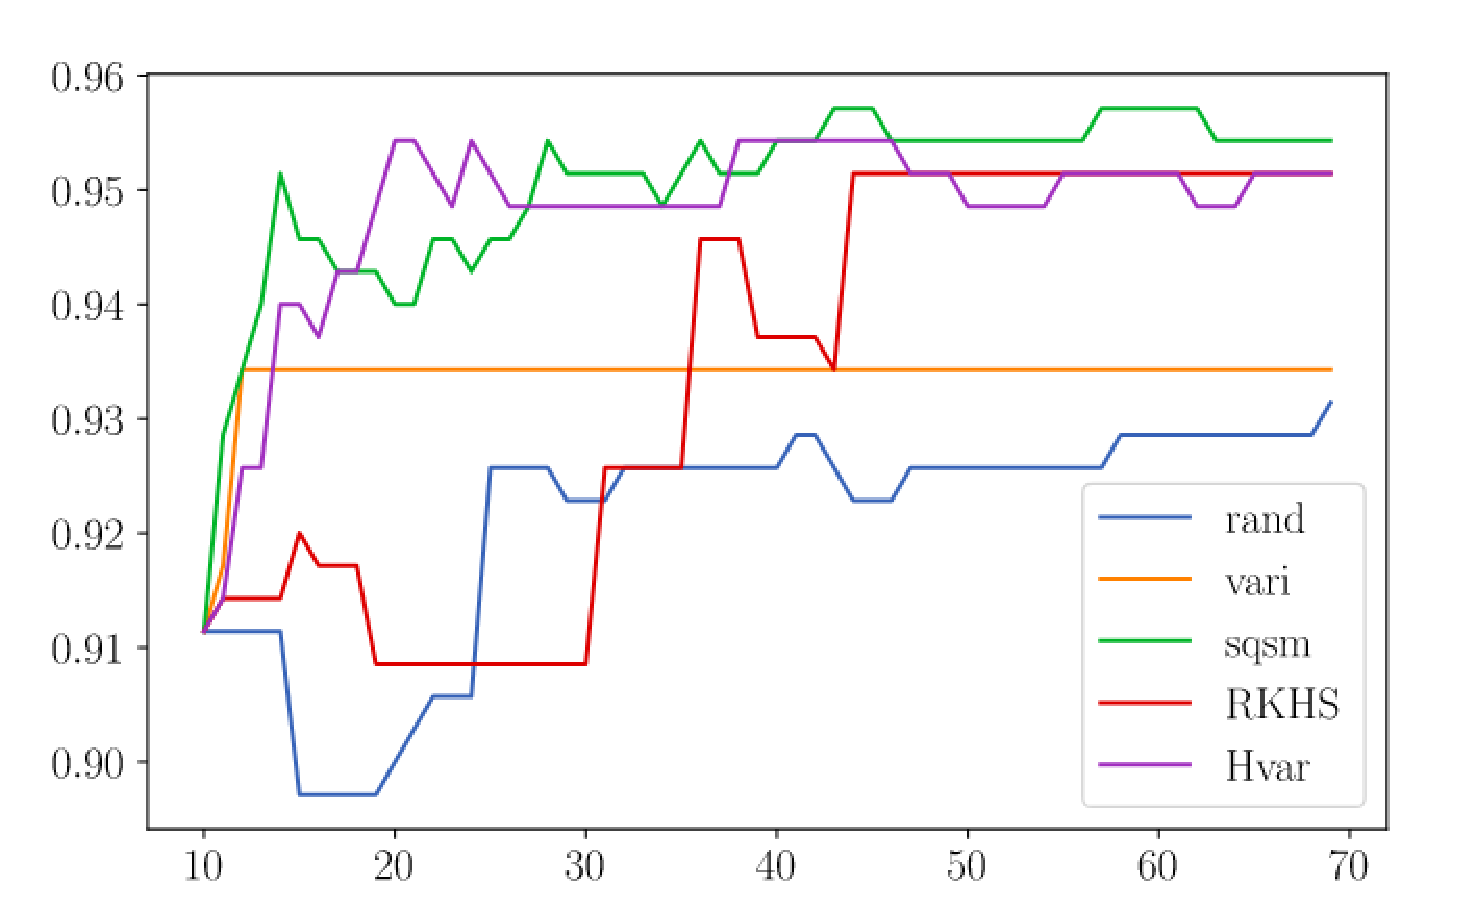
\includegraphics[scale = 0.4]{acc1dim.eps}}
\caption{Графики точности классификации на отложенной выборке в зависимости от размера обучающей выборки для одномерных данных.}
\label{acc1dim}
\end{figure}
На рис. \ref{scoreplots} изображены графики $score$-функций на одной из итерации алгоритма активного обучения для этих методов. На графики так же добавлены вероятности принадлежности точек $x$ к классу 1. Это позволяет заметить, что локальные максимумы расположены близко к границам разделения классов.
\vspace*{-0.5cm}
\begin{figure}[h]
\begin{minipage}[h]{0.49\linewidth}
\center{\includegraphics[scale = 0.8]{11.eps}}
\end{minipage}
\hfill
\begin{minipage}[h]{0.49\linewidth}
\center{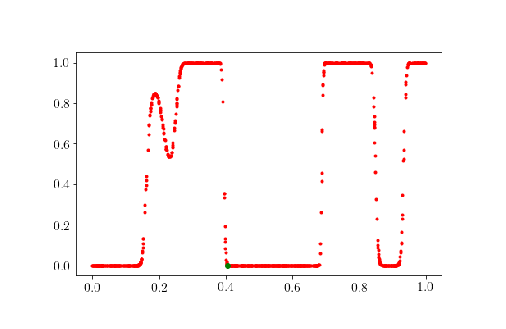
\includegraphics[scale = 0.8]{1.eps}}
\end{minipage}
\vfill
\begin{minipage}[h]{0.49\linewidth}
\center{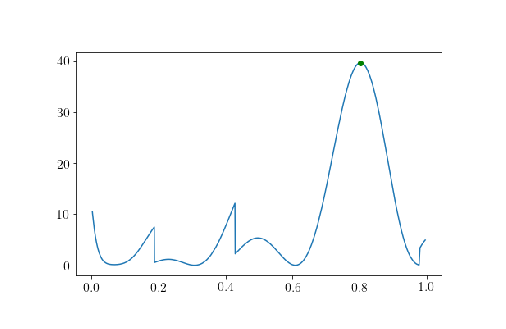
\includegraphics[scale = 0.8]{12.eps}} Hvar
\end{minipage}
\hfill
\begin{minipage}[h]{0.49\linewidth}
\center{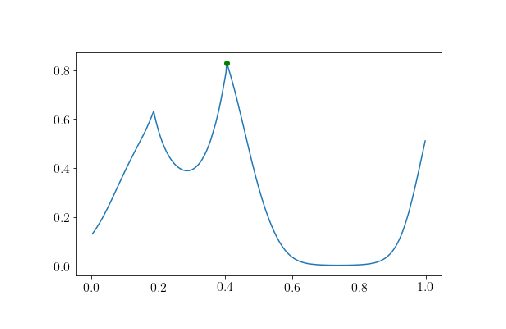
\includegraphics[scale = 0.8]{2.eps}} sqsm
\end{minipage}
\caption{Графики $score$-функций на одной из итерации алгоритма активного обучения. На верхних рисунках изображены вероятности принадлежности точек на оси $x$ к классу 1. Зеленые точки обозначают точку с максимальным значением $score$-функции. Нижние рисунки иллюстрируют значения $score$-функций, соответствующие двум методам: Hvar (слева) и sqsm (справа).}
\label{scoreplots}
\end{figure}
\begin{comment}
\begin{figure}[h]
\begin{minipage}[h]{0.49\linewidth}
\center{\includegraphics[scale = 0.4]{score_sqsm.eps} \\ 1) sqsm}
\end{minipage}
\hfill
\begin{minipage}[h]{0.49\linewidth}
\center{\includegraphics[scale = 0.4]{score_Hvar.eps} \\ 2) Hvar}
\end{minipage}
\caption{Графики $score$-функций. По горизонтальной оси расположены $x$ - точки исходного датасета. По вертикальной оси отложены значения $score$-функции. Для наглядности добавлены красные точки -- вероятности принадлежности точки на горизонтальной оси классу 1. Синия линия -- график $score$-функции. Вертикальная прямая соответсвует точке максимума $score$-функций и, соответственно, следующей точке, метку которой хочет узнать модель.}
\end{figure}
\end{comment}
%\vspace*{-1cm}
\subsubsection{Многомерные синтетические данные} Для задачи бинарной классификации были сгенерированы 5-мерные данные. Аналогичным образом построены графики точности классификации в зависимости от размера обучающей выборки, представленные на рис. \ref{acc5dim}. Здесь лучше всего работают методы RKHS и Hvar.
\begin{figure}[h]
\vspace{0 cm}
\center{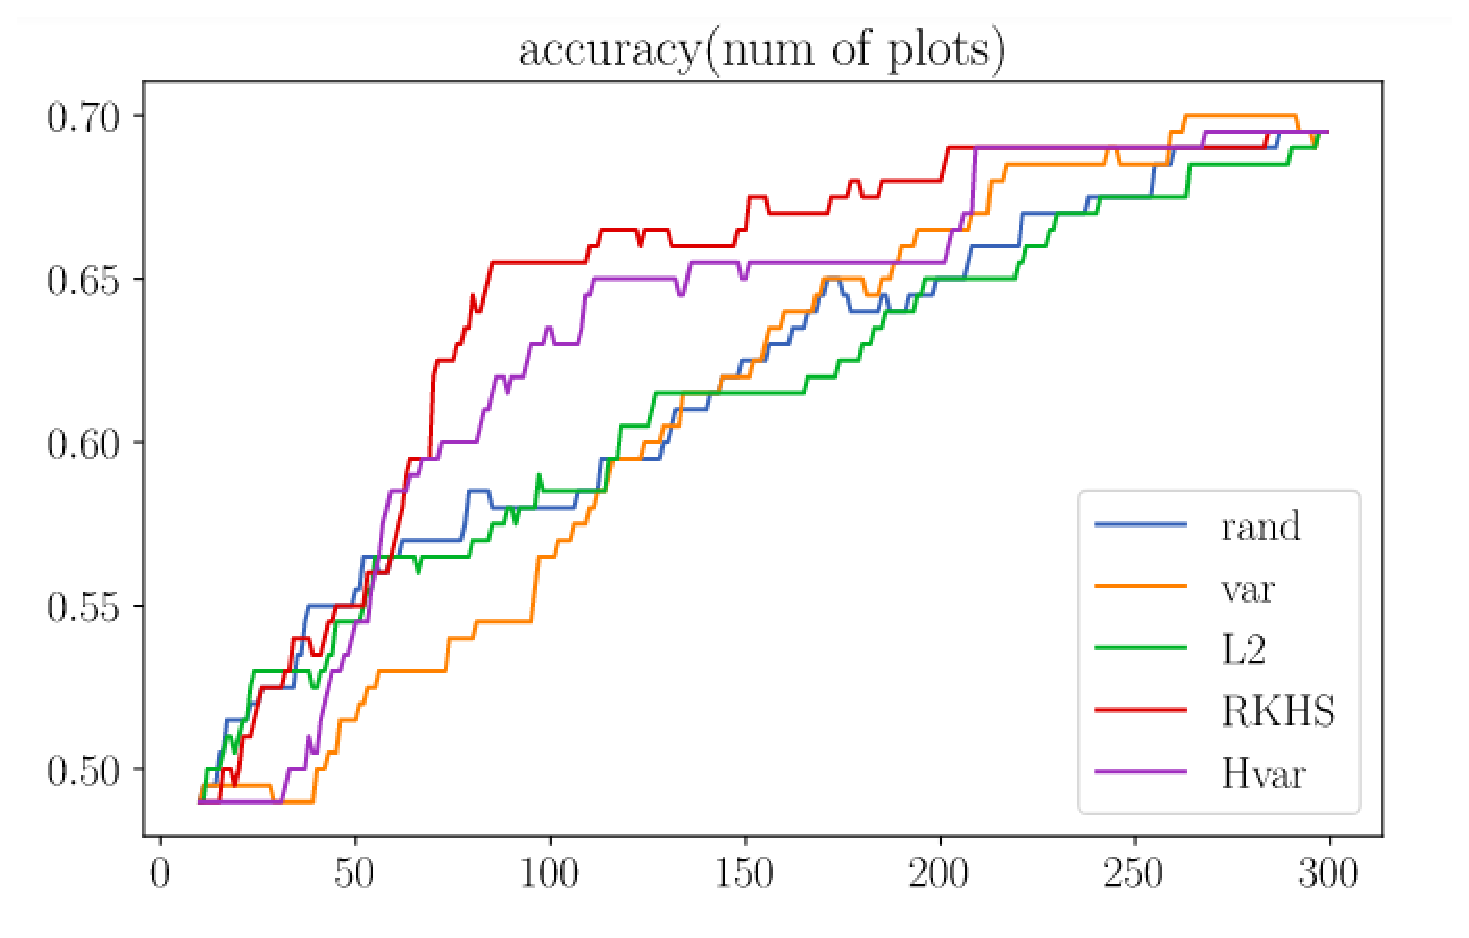
\includegraphics[scale = 0.4]{acc5dim.eps}}
\caption{Графики точности классификации на отложенной выборке в зависимости от размера обучающей выборки для 5-мерных данных.}
\label{acc5dim}
\end{figure}

%/* Реальные датасеты - банкноты и пульсары (если экперименты досчитаются) \\
%Более того, я боюсь, будут ли вообще приемлимыми результаты */\\
\section{Заключение}
В этой работе мы рассмотрели применение гауссовских процессов к задаче классификации и различные варианты алгоритмов активного обучения и сравнили их качество. Нам так же удалось посмотреть на их работу "изнутри" \ с помощью графиков $score$-функций. По имеющимся результатам можно сказать лишь, что в условиях, когда данных мало, хорошо работают методы sqsm, RKHS и Hvar. Причем последний хорошо показывает себя в обоих рассмотренных задачах. Первый же имеет наиболее наглядную интерпретацию в плане графиков $score$-функций.\\
Заметим, что ранее таким сравнением методов никто не занимался. В дальнейшем, безусловно, планируется поставить более масштабные эксперименты, т.к. небольшой размер тестовой выборки вызывает дискретность значний точности, из-за чего графики трудно воспринимать.
%\newpage	
\begin{thebibliography}{}

\bibitem[1]{av}
Mina Karzand, Robert D. Nowak:
Active Learning in the Overparameterized
and Interpolating Regime
arXiv preprint arXiv:1905.12782,2019

\bibitem[2]{gp}
C. E. Rasmussen, C. K. I. Williams, 
Gaussian Processes for Machine Learning, 
the MIT Press, 2006, ISBN 026218253X

\bibitem[3]{approximations}
Hannes Nickisch, Carl Edward Rasmussen, 
Approximations for Binary Gaussian Process Classification, 
Journal of Machine Learning Research 9 (2008) 2035-2078 

\bibitem[4]{teorver}
Гнеденко Б. В., 
Курс теории вероятностей, 
УРСС. М.: 2001

\bibitem[5]{overparam}
Siyuan Ma, Raef Bassily, and Mikhail Belkin. 
The power of interpolation: Understanding the effectiveness of sgd in modern over-parametrized learning. 
In International Conference on Machine Learning, pages 3331–3340, 2018.

\bibitem[6]{generalav}
Burr Settles. 
Active Learning Literature Survey.  
2010.

\bibitem[7]{uncertainty}
D. Lewis and W. Gale. 
A sequential algorithm for training text classifiers. 
In Proceedings of the ACM SIGIR Conference on Research and Development in Information Retrieval, 
pages 3–12. ACM/Springer, 1994.

\bibitem[8]{comitee}
H.S. Seung, M. Opper, and H. Sompolinsky. 
Query by committee. In Proceedings of the ACM Workshop on Computational Learning Theory,
pages 287–294, 1992

\bibitem[9]{Hvar}
Burnaev E., Panov M. (2015) 
Adaptive Design of Experiments Based on Gaussian Processes. In: Gammerman A., Vovk V., Papadopoulos H. (eds) Statistical Learning and Data Sciences. SLDS 2015. 
Lecture Notes in Computer Science, vol 9047. Springer, Cham


\bibitem[10]{minnorm}
Trevor Hastie, Andrea Montanari, Saharon Rosset, and Ryan J Tibshirani. 
Surprises in high-dimensional ridgeless least squares interpolation. 
arXiv preprint arXiv:1903.08560, 2019.

\end{thebibliography}
\end{document}
